\section{Results}

\subsection{The Model}

In this work, we present a probabilistic generative model for single-molecule image-data and describe Bayesian inference approach used to obtain posterior distributions of latent model parameters. The generative model can be interpreted as a causal process that produces the observed image data. The graphical model in Figure 2A visually describes latent variables of the model and conditional independence structure of the model. We model the observed image as ``spot'' images of binder molecules superimposed on background image. Fluorescence spots are modeled as a 2D Gaussians parameterized by a set of variables ($h, w, x, y$) which accurately approximates fluorescence microscope point spread function \cite{Zhang2007-rb}. The model depends on various unobserved physical parameters such as background photon intensity and the number, position, shape, and intensity of each spot in the image. The unobserved parameters, in turn, are described by prior distributions which embed into the model our existing knowledge of the experiment, such as the likely position of an on-target spot. Explicitly model on-target and off-target spots.

Our model assumes that at maximum 2 spots in total can be present in a single image and at maximum only one on-target spot. The image model described above allows to capture many of the characteristics of real experimental data, such as site and time dependent fluctuations in the local background signal, time dependent fluctuations in the spot intensity and its position, simultaneous binding of on-target and off-target spots, Gamma distributed noise, which is more realistic than Gaussian noise. Figure 2B,C,D shows examples where there is no spot, one spot, or two spots and corresponding spot parameters in the table.

Total observed intensity is the sum of the offset signal (dark current) plus the photon counts amplified by the gain setting of the camera. The linear relationship between the noise variance and the mean intensity is built into the intensity model through the gain and offset parameters and the gain parameter is fitted along with other parameters. Distribution of the offset signal is obtained as a histogram density signal from the single-molecule images (Figure ).  In Figure we show raw images and their intensity distributions along with the images simulated from the posterior distribution (posterior predictive checking). Comparison of images and distributions for spot/no spot cases show that our model accurately models intensity as a function of mean intensity reflecting the dependence of the noise on the mean intensity. Additionally, Figure shows that the gain parameter is accurately inferred for a simulated set of data with varying gain parameter where the true value of the gain parameter is known.

\subsection{Bayesian Inference and Implementation}

Posterior distributions of latent variables conditioned on the observed data is given by the Bayes' theorem. The evidence in general is intractable. Here we use stochastic variational inference (SVI) approach and maximize the evidence-lower bound (ELBO). Our program Tapqir is open-source (github link) and is implemented in the probabilistic programming language Pyro. The advantage of using PPL like Pyro is its black box SVI approach which allows to focus on the model, efficient computation on GPU, scalability to large datasets. Details of the generative model and variational model are given in the online Methods section.

\subsection{Analysis of simulated data}

As a validation of our model we demonstrate its application to simulated synthetic data. Fake-data simulation is important because it allows to directly check that the inference on latent variables is reliable. Thus, fake-data simulation provides an upper bound of what can be learned reliably about the model for various types of data. Simulation parameters details are described in the online Methods. We made 10 randomized simulations and then fit the synthetic data to the model. Figure 3 shows plots of the simulated values of the global parameters (gain, average on-target spot probability, average off-target spot probability, proximity) vs the fitted values. The results demonstrate that model parameters can be reliably recovered which is good.

MCC plot. Example traces.

\subsection{Analysis of experimental data}

Thermodynamic Analysis.

In this section, we describe different aspects of our model. The Bayesian model described here is holistic in a sense that the observed data and all of the model parameters are interconnected. However, its modular structure allows to view and analyze different parts of the model separately. Below we review briefly the CoSMoS method and the type of data generated by CoSMoS experiments, and then describe the image model, the intensity model, spot-detection, and co-localization aspects of the model.

\subsection{Multi-wavelength single-molecule co-localization methods}

Before describing the approach used for the analysis of CoSMoS data, it is helpful to  review briefly the experimental method. The key features of a CoSMoS experiment include: 1) One species of fluorescently labeled molecule (called the “target”) is tethered to the surface of the observation chamber. Target molecules are immobilized at a surface density sufficiently low that the mean nearest-neighbor distance is large relative to the point-spread function (i.e., the diffraction-limited spot size) of the microscope. 2) Molecules, each species labeled with a different dye color, are added to the solution over the surface, typically at concentrations $\leq 1 \mu$M. When these “binder” molecules are freely diffusing in solution, they are invisible in TIRF. In contrast, when they are bound to the target, single binder molecules are detected as discrete fluorescent spots (Figure \ref{fig:cosmos_experiment}). The combination of features 1 and 2 means that formation of an individual binder-target complex is detected as spot appearance; dissociation of a binder-target complex is detected as spot disappearance \cite{Friedman2006-kb, Friedman2015-nx}.

\subsection{CoSMoS image data}

CoSMoS data analysis requires identifying the locations of target molecules and the corresponding positions in the binder molecule camera channel. Image pre-processing steps include alignment of images from multiple wavelength channels and drift correction \cite{Friedman2015-nx, Smith2019-yb}. Single-molecule images after pre-processing steps consists of a $P \times P$ matrix of pixel intensities with the target molecule at the center of the image. One experiment typically consists of a set of images where we have $N$ target sites ($n \in \{1,\dots,N\}$) each consisting of a series of $F$ different images in a recording ($f \in \{1,\dots,F\}$) (a “recording”).

CoSMoS images consist of offset signal, background intensity and diffraction-limited spots. Detection of on-target binding depends on the intensity of the spot and its distance to the target molecule. The size $P=14$ of the selected area is chosen to be large enough to detect the on-target spot and reliably determine the local background intensity. In addition to the on-target spot, non-specifically bound binder molecules can also be present in the image. Usually no more than two spots are present in the single image. Frequently, identification of on-target binding is complicated by molecules binding off-target which distort the shape of the on-target spot and its apparent distance to the target. 

%\begin{figure}
%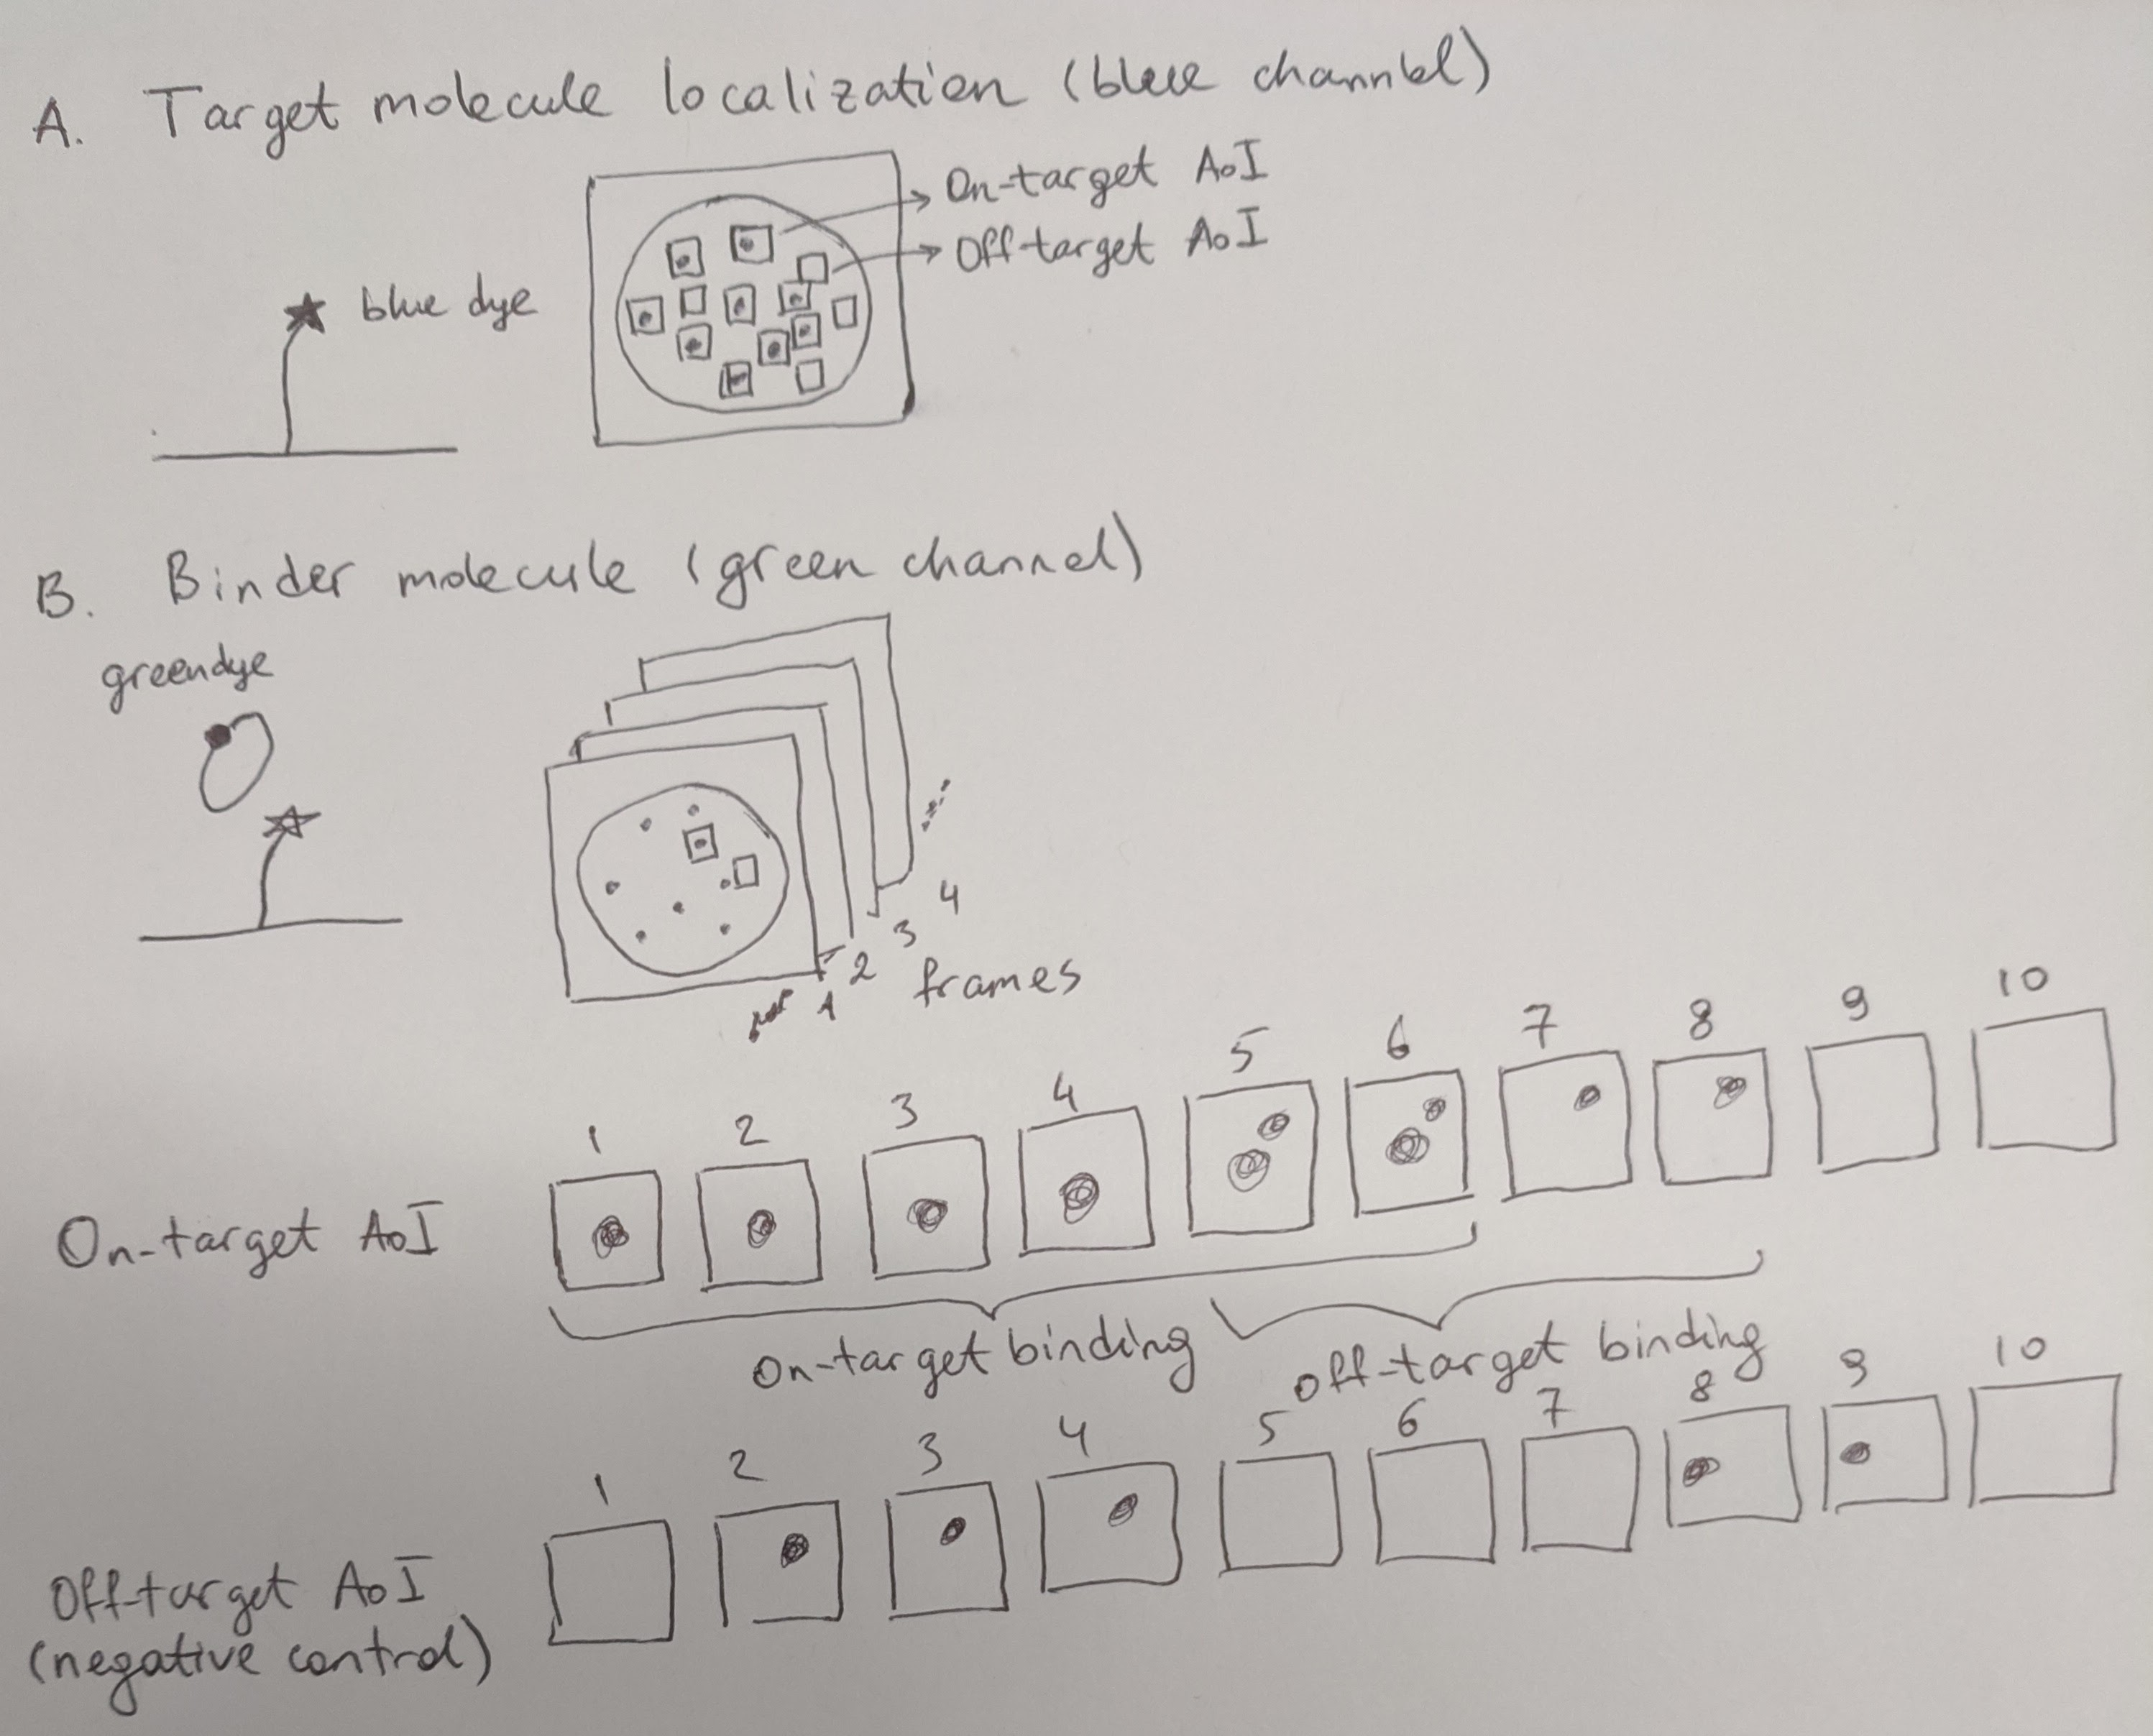
\includegraphics[width=\linewidth]{figures/figure1.jpg}
%\caption{Co-localization single molecule spectroscopy experiment. (A) Target molecules are localized in the blue channel and then on-target and off-target areas of interest are selected. (B) Movies of the binder molecule collected in the green channel. In selected AoI binder molecules can be on-target, off-target, or absent.}
%\label{fig:cosmos_experiment}
%% If the optional argument in the square brackets is "none", then the caption *will not appear in the main figure at all* and only the full caption will appear under the supplementary figure at the end of the manuscript.
%\figsupp[Shorter caption for main text.]{This is a supplementary figure's full caption, which will be used at the end of the manuscript.}{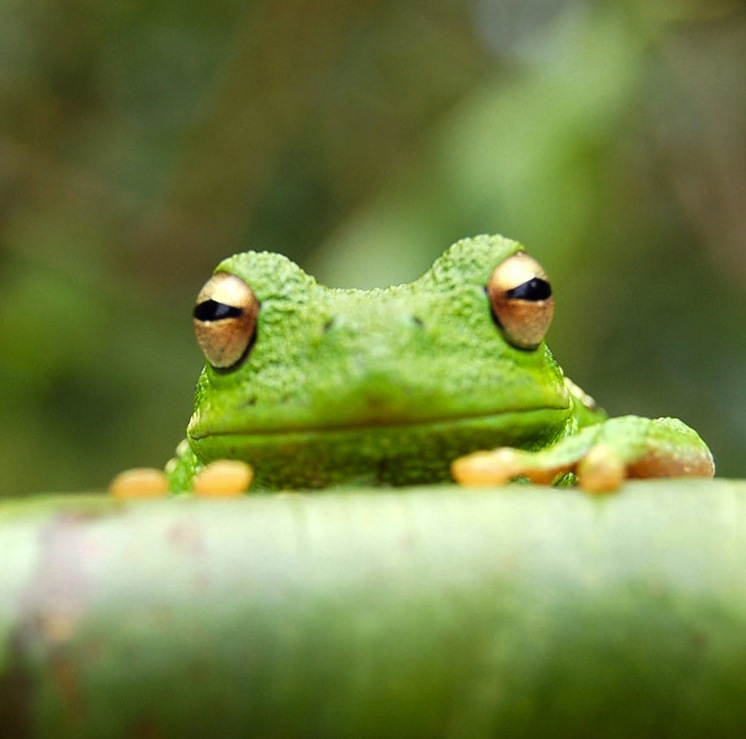
\includegraphics[width=6cm]{frog}}\label{figsupp:sf1}
%\figsupp{This is another supplementary figure.}{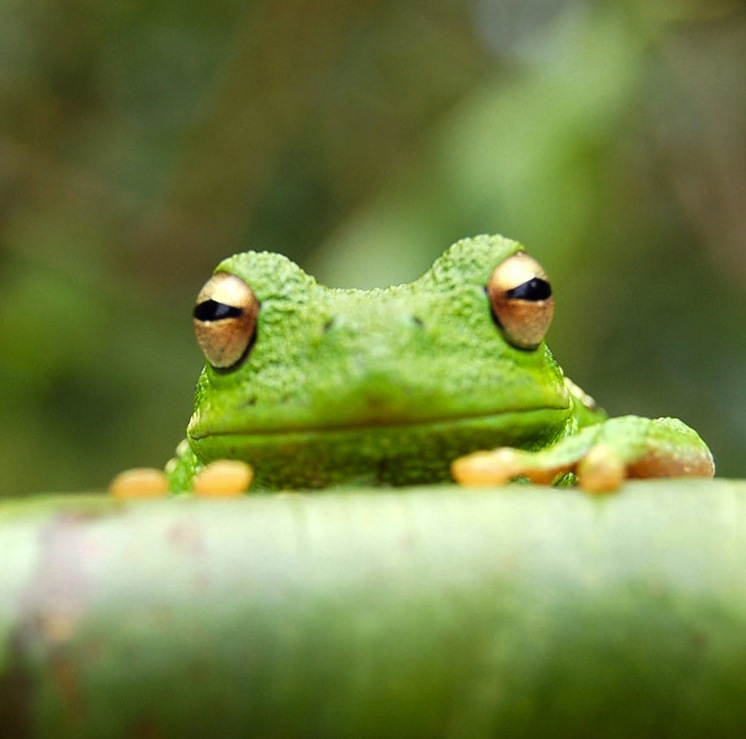
\includegraphics[width=6cm]{frog}}
%\figdata{This is a description of a data source.}\label{figdata:first}
%\figdata{This is another description of a data source.}\label{figdata:second}
%\end{figure}

%\begin{figure}
%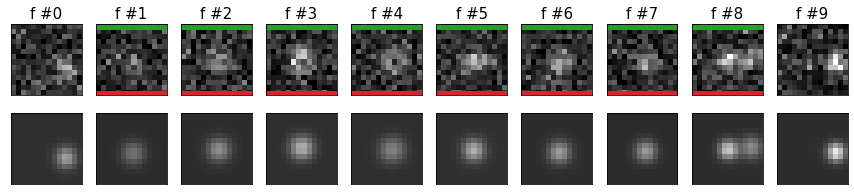
\includegraphics[width=\linewidth]{figures/figure3a.png}
%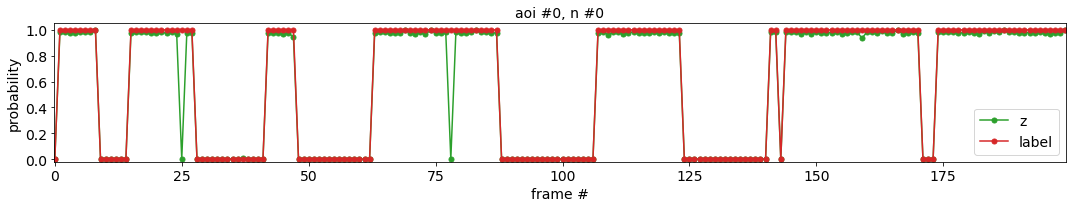
\includegraphics[width=\linewidth]{figures/figure3b.png}
%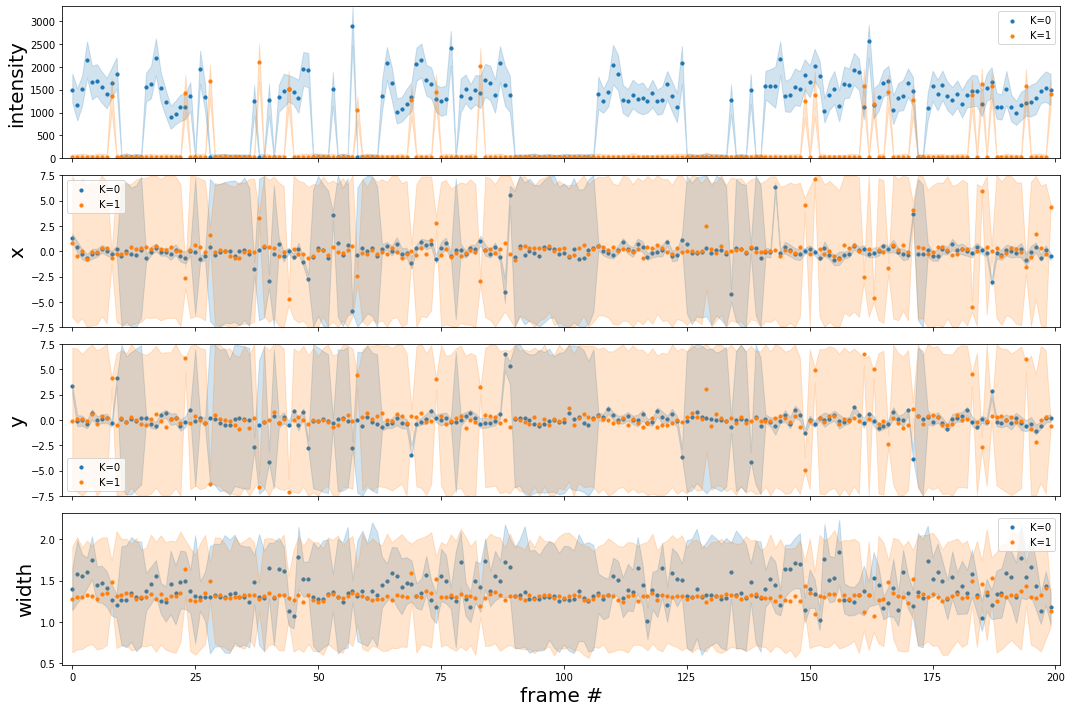
\includegraphics[width=\linewidth]{figures/figure3c.png}
%\caption{Co-localization single molecule spectroscopy experiment. (A) Target molecules are localized in the blue channel and then on-target and off-target areas of interest are selected. (B) Movies of the binder molecule collected in the green channel. In selected AoI binder molecules can be on-target, off-target, or absent.}
%\label{fig:view}
%\end{figure}

\subsection{Image Model Module} 

We model the observed image as ``spot'' images of binder molecules superimposed on background image. In particular, background image consists only of constant background intensity $\mathrm{b}_{nf}$ that can vary from image to image. Our model assumes that at maximum $K=2$ number of spots can be present in a single image.  Fluorescence spot is modeled as a 2D Gaussian which accurately approximates fluorescence microscope point spread function \cite{Zhang2007-rb}. Each spot is parameterized by integrated scalar intensity $\mathrm{h}_{nfk}$, width $\mathrm{w}_{nfk}$, and relative position $\mathrm{x}_{nfk}$ and $\mathrm{y}_{nfk}$ to the target molecule. All of the spot parameters are local/individual for each spot.

We use binary indicator variable $\mathbf{m} = \{\mathrm{m}_{nfk}\}$ to denote the presence of each individual spot ($k \in \{1,\dots,K\}$). The value of the index variable $\theta_{nf} \in \{0,1,\dots,K\}$ specifies the index of the on-target spot when it is present and equals zero when the on-target spot is absent. There are $2^K + K2^{K-1}$ unique combinations of $\mathrm{m}$ and $\theta$ which define the state space for each image. Table~\ref{tab:states} shows the state space when $K=2$. Thus, we get the image model ($\mu^I_{nfij}$) calculated as the sum of the background intensity ($\mathrm{b}_{nf}$) and 2D Gaussian spots ($\mu^S_{knfij}$) present in the image.

\subsection{Spot Detection}

WIP

Spot detection is performed in a probabilistic manner. Spot existence probability depends on the information in the entire image. However, it primarily correlates with the intensity of the spot. Discrimination of spots from random fluctuations in the background signal depends on the prior and not on the threshold parameter. In the absence of prior information uninformative prior can be used. Plotting results show that with half normal prior spots have to be roughly above 1 SNR.

\subsection{Co-localization}

For the spots that are present in the image they can be further classified as on-target (co-localization) or off-target (non-specific). The probability of being on-target or off-target is dictated primarily by the distance to the target. Spots bound on-target and off-target have different prior distributions of their location relative to the target molecule. This prior knowledge is used to discriminate between on- and off-target spots in a probabilistic manner using mixture distributions model. Off-target spots have a uniform prior distribution across the image and can bind anywhere on the surface with equal probability. On-target spots, on the other hand, are clustered near the target molecule. Standard deviation of the distribution of on-target spots depends on the spot localization accuracy and the mapping accuracy between target and binder channels (?). By analyzing simulated data we have established that this parameter, also called the proximity parameter, can be reliably determined by floating it during the fit (Figure ). Alternatively, proximity parameter can be determined experimentally and fixed in the model. Figure show the distribution of the center of mass of on-target spots which are tightly clustered around the target molecule. On the other hand, off-target spots are distributed more uniformly across the area of the image.

Second, the posterior probabilities of being classified as on-target or off-target spot depends on the prior average frequencies of on-target and off-target spots. Increasing the ratio of the off-target molecules to on-target molecules decreases the probability of the spot being on-target reflecting the fact that.

This standard distribution can be determined independently and used as a fixed parameter in the model. However, it can also be floated in the fit and determined from the overall distribution of the center of masses of spots. $\sigma^{xy}$, $\pi^z$, and $\lambda^j$ are correlated. Figure shows simulated data with varying parameters where the true values of parameters are inferred correctly. Note that the posterior probability of the spot class depends on its relative position to the target and average probabilities of on-target and off-target spots.

\subsection{Informal Kinetic/Thermodynamic Analysis}

WIP